\documentclass[11pt, a4paper, oneside]{memoir}                                                      %%

\usepackage[utf8]{inputenc}
\usepackage[ngerman]{babel}     % new german spelling, umlauts and other regional settings like date format
\usepackage[shortlabels]{enumitem}
\usepackage{nameref,zref-xr}
\zxrsetup{toltxlabel}
\usepackage{graphicx}           % allow for inclusion of images
\usepackage[table,svgnames]{xcolor} % define colors
\usepackage{url}                % weblinks, etc.
\usepackage{colortbl}           % colored table cells
\usepackage{longtable}          % tables, which are longer than one page
\usepackage{hyperref}
\usepackage[intlimits]{mathtools}
\hypersetup{
	bookmarksopen=true,                       % expand bookmark tree in acrobat by default
	pdftitle={SEPMP},                         % set title in meta pdf information
	pdfauthor={Teilnehmer 1, Teilnehmer 2, Teilnehmer 3},                             % set author in meta pdf information
	pdfsubject={},                            % set subject in meta pdf information
	pdfkeywords={},                           % set keyword list in meta pdf information
	colorlinks=true,                          % use colored links instead of black ones
	linkcolor=blue,                           % color for internal links
	anchorcolor=black,                        % color for anchor links
	citecolor=black,                          % color for bibliography links
	filecolor=magenta,                        % color for system local links
	urlcolor=blue,                            % color for url links
	plainpages=false,                         % must be false, so that PDF bookmarks work properly
	hypertexnames=false,                      % use guessable names for links; used for correct bookmarks
	linktocpage                               % link page numbers in toc instead of section names
}
\makeatletter
\def\namedlabel#1#2{\begingroup
    #2%
    \def\@currentlabel{#2}%
    \phantomsection\label{#1}\endgroup
}
\makeatother

\newenvironment{lhp}[3]%
{%
	\item [\namedlabel{#3}{/#2\arabic{#1}/}]% \hfill%
	\addtocounter{#1}{10}%
	\begin{description}[leftmargin=0cm, style=sameline]%
}%
{%
	\end{description}%
}

\newenvironment{php}[4]%
{%
	\item [\namedlabel{#4}{/#2\arabic{#1}/} (\ref{#3})] \hfill%
	\addtocounter{#1}{10}%
	\begin{description}[style=sameline]%
}%
{%
	\end{description}%
}

\makeatletter
	\newcommand{\mysubject}{Lastenheft}
	\newcommand{\mygroup}{}
	\newcommand{\myauthor}{%
			Lukas Bayer \\
			Nils Fitting \\
 			Marco Tücks \\
 			Alexander Wilhelm \\
 			Lukas Tuchtenhagen %
 			}
\makeatother

\begin{document}

	\thispagestyle{empty}
	\newcommand{\Rule}{\rule{\textwidth}{0.5mm}}
	\begin{center}
	% upper part
	{\Large 
\includegraphics[height=20mm]{img/TUKL_LOGO_4C} \par}

	\vspace{0.5em}

	{\Large AG Computergrafik \& HCI \\ apl. Prof. Dr. Achim Ebert \par}

	\vspace{0.5em}

	{\Large SEP/MP \the\year \par}


	\vspace{5cm}

	% middle part
	\Rule

	\vspace{1cm}

	{\Huge Ablauf der Präsentation \par}

	\vspace{0.5em}

	{\Large \mysubject \par}

	\vspace{0.5em}

	{\small \today \par}

	\vspace{0.7cm}

	\Rule


	\vfill %%%%%%%%%%%%%%%%%%%%%%%%%%%%%%%%%%%%%%%%%%%%%%%%%%%%%%%%%%%%%%%%


	% lower part
	\emph{\textbf{\mygroup}} \\[1em]
	\myauthor

	\end{center}


	\tableofcontents

	\chapter{Projekttreiber}

\section{Projektziel}

Im Rahmen des Software-Entwicklungs-Projekts/Modellierungspraktikums {\the\year} soll ein einfach zu bedienendes Client-Server-System zum Spielen von Bohnanza über ein Netzwerk implementiert werden. Die Benutzeroberfläche soll intuitiv bedienbar sein.

\section{Stakeholders}

\newcounter{sh}\setcounter{sh}{10}

\begin{description}[leftmargin=5em, style=sameline]
	
	\begin{lhp}{sh}{SH}{sh:Spieler}
		\item [Name:] Spieler
		\item [Beschreibung:] Menschliche Spieler.
		\item [Ziele/Aufgaben:] Das Spiel zu spielen.
	\end{lhp}
	
	\begin{lhp}{sh}{SH}{bsh:Spieler}
		\item [Name:] Eltern
		\item [Beschreibung:] Eltern minderjähriger Spieler.
		\item [Ziele/Aufgaben:] Um die Spieler zu kümmern, indem Eltern Spielzeit begrenzen wollen und zugriff auf sensible Inhalte begrenzen.
	\end{lhp}
	
	\begin{lhp}{sh}{SH}{bsh:gesetzgeber}
		\item [Name:] Gesetzgeber
		\item [Beschreibung:] Das Amt für Jugend und Familie.
		\item [Ziele/Aufgaben:] Die Rechte der Spieler zu schützen und zu gewähren, indem er Gesetze erstellt.
	\end{lhp}
	
	\begin{lhp}{sh}{SH}{bsh:investor}
		\item [Name:] Investoren (nur für Beispielzwecken)
		\item [Beschreibung:] Parteien, die das Finanzmittel für die Entwicklung des Systems bereitstellen.
		\item [Ziele/Aufgaben:] Gewinn zu ermitteln, indem das System an Endverbraucher verkauft wird.
	\end{lhp}
	
	\begin{lhp}{sh}{SH}{bsh:betreuer}
		\item [Name:] Betreuer
		\item [Beschreibung:] HiWis, die SEP/MP Projektgruppen betreuen.
		\item [Ziele/Aufgaben:] Das Entwicklungsprozess zu betreuen, zu überwachen und teilweise zu steuern als auch die Arbeit der Projektgruppen abzunehmen sowie den Studenten im Prozess Hilfe zur Verfügung zu stellen. 
	\end{lhp}
	
	\begin{lhp}{sh}{SH}{bsh:prof}
		\item [Name:] Prof. Dr. Achim Ebert
		\item [Beschreibung:] Betreuer des Gesamtprojekts 
		\item [Ziele/Aufgaben:] Als zentraler Ansprechpartner betreut er in Zusammenarbeit mit den HiWis das Projekt und bewertet es schlussendlich.
	\end{lhp}
		
\end{description}

\section{Aktuelle Lage}

Aktuell wird Bohnanza als Familien-Kartenspiel verwendet und besitzt (für seine Originalvariante) keine technisch realisierte Anwendung. Es sind diverse Erweiterungen, wie auch Spin-Offs des Titels erschienen, auf die in diesem Projekt aus zeitlichen Gründen nicht weiter eingegangen wird. Für uns ist es wichtig, eine solide Alternative zum klassischen Kartenspiel zu entwerfen, die dem Original durch angemessene Musik, Grafik und Interaktion neue Farbe verleiht. \\
Im weiteren Verlauf sind weder Erweiterungen noch Online-Varianten geplant.
	\chapter{Projektbeschränkungen}

\section{Beschränkungen}

\newcounter{lb}\setcounter{lb}{10}

\begin{description}[leftmargin=5em, style=sameline]
	
	\begin{lhp}{lb}{LB}{beschr:lehrbots}
		\item [Name:] Selbstlehrende Bots
		\item [Beschreibung:] Keine Selbstlehrfunktion von Bots wird implementiert.
		\item [Motivation:] Die Funktionalität ist zu aufwändig zu implementieren und passt deshalb nicht in das Zeitbudget.
		\item [Erfüllungskriterium:] Intelligenzalgorithmus von Bots ist so vorprogrammiert, dass sie Entscheidungen nur anhand des vorprogrammierten Wissens sowie des aktuellen Spielstands treffen, ohne dabei frühere Spiele zu berücksichtigen.
	\end{lhp}
	
	\begin{lhp}{lb}{LB}{beschr:anwendungsbereich}
		\item [Name:] Anwendungsbereich
		\item [Beschreibung:] Das System ist ausschließlich für den privaten Bereich ausgelegt.
		\item [Motivation:] Im Laufe des Projekts muss die Software lediglich privat getestet und vorgeführt werden.
		\item [Erfüllungskriterium:] Das Programm kann fehlerfrei vorgeführt werden.
	\end{lhp}
	
		
	\begin{lhp}{lb}{LB}{beschr:implsprache}
		\item [Name:] Implementierungssprache
		\item [Beschreibung:] Für die Implementierung ist ausschließlich Java 8 oder höher zu verwenden.
		\item [Motivation:] Das optimiert die Betreuung von SEP/MP und koordiniert die Mitarbeit.
		\item [Erfüllungskriterium:] Die Software wurde einheitlich mittels Java 8 implementiert.
	\end{lhp}
	
	\begin{lhp}{lb}{LB}{beschr:gui}
		\item [Name:] GUI-Framework
		\item [Beschreibung:] Die GUI ist mit JavaFX zu realisieren.
		\item [Motivation:] Das optimiert die Betreuung von SEP/MP und koordiniert die Mitarbeit.
		\item [Erfüllungskriterium:] Fenster und ihre Funktionen sind für die Nutzer intuitiv gestaltet und somit von von Spieler einfach zu bedienen.
	\end{lhp}
	
	\begin{lhp}{lb}{LB}{beschr:gitlab}
		\item [Name:] Gitlab
		\item [Beschreibung:] Für die Entwicklung ist das vorgegebene GitLab-Repository zu verwenden.
		\item [Motivation:] Das optimiert die Betreuung von SEP/MP und koordiniert die Mitarbeit.
		\item [Erfüllungskriterium:] Die Struktur und Interaktion zwischen den Softwareabschnitten wurde bereits frühzeitig in der Architektur festgehalten.
	\end{lhp}
	
	
\end{description}

\section{Glossar}

\begin{center}
		\rowcolors{2}{Gray!15}{White}
		\begin{longtable}{p{0.25\textwidth} p{0.25\textwidth} p{0.4\textwidth}}
			\textbf{Deutsch} & \textbf{Englisch} & \textbf{Bedeutung} \\
			\hline \hline \endhead                   
			Bot & bot & Spieler, dessen Spielaktionen vom Computer entschieden und durchgeführt werden\\
			Kekse & Cookies & Offiziell keine gültige Maßnahme zur Bestechung der HiWis\\          
 			Lobby & lobby & Virtueller Raum zum Betreten eines Spielraums\\	
			Spiel (Regelwerk) & game & Bohnanza \\
			Spieler & player & Teilnehmer am Spielgeschehen\\
			Spielraum & game room & Virtueller Raum, in dem ein Spiel stattfindet\\
			Zug & turn & Zustand in dem ein Spieler eine Spielaktion ausführen muss\\
			Spin-off & spinoff & Eigenständiges Spiel mit grundlegender Abwandlung des originalen Spielprinzips \\
			Bohne & bean & Bezeichnung für die in verschiedene Kategorien eingeteilten Spielkarten\\
			Taler & thaler &  Eine Währung im Spiel\\
			Bohnenfeld & field & Ablage, auf der Bohnen im Spielverlauf "angebaut" werden\\
			Hand & hand & Karten, die der Spieler in der Hand hält\\
			Bohnenhandel & bean trading & Möglichkeit der Spieler innerhalb bestimmter Spielphasen Karten miteinander zu 					tauschen\\
			Bohnenschutzregel & bean protection policy & Eine Regel, die das Abbauen von Bohnen vom Feld einschränkt		
		\end{longtable}
\end{center}

\section{Relevante Fakten und Annahmen}

Wichtige gekannte Fakten und getroffene Annahmen, die sich auf das Projekt direkt oder indirekt beziehen und dadruch auf die zukünftige Implementierungsentscheidungen Effekt haben können.

\newcounter{fa}\setcounter{fa}{10}

\begin{description}[leftmargin=5em, style=sameline]
	
	\begin{lhp}{fa}{FA}{fa:fortentwicklung}
		\item [Name:] Keine Fortentwicklung des App nach SEP/MP.
		\item [Beschreibung:] Nach Ende des SEP/MP wird das Projekt nicht weiterentwickelt.
		\item [Motivation:] Das Entwicklungsteam hat keinen Bock darauf.
	\end{lhp}
	
	\begin{lhp}{fa}{FA}{fa:recht}
		\item [Name:] Keine Lizenzen für Spielartefakte.
		\item [Beschreibung:] Weder TU Kaiserslautern noch die Spielwerk + Freizeit GmbH gewahren dem Entwicklungsteam die Rechte für die Spielartefakte.
		\item [Motivation:] Rechtliche Vorsorge.
	\end{lhp}
	
	\begin{lhp}{fa}{FA}{fa:recht-vergangenheit}
		\item [Name:] Keine bekannte Nachteile von Verwendung von Spielartefakten.
		\item [Beschreibung:] Es ist nicht bekannt, dass die SEP/MP-Teilnehmer der letzten Jahre irgendwelche rechtliche Probleme dadurch gehabt haben, dass sie die Speilartefakten von Spielwerk + Freizeit GmbH im Rahmen ihrer SEP/MP eingesetzt haben.
		\item [Motivation:] Rechtliche Vorsorge.
	\end{lhp}
	
	
\end{description}


	\chapter{Funktionale Anforderungen}

%\section{Systemkontext}

\section{Systemfunktionen}

\newcounter{pfc}\setcounter{pfc}{10}

\begin{description}[leftmargin=5em, style=sameline]
	
	\begin{lhp}{pfc}{LF}{funk:spielverw}
		\item [Name:] Spielverwaltung
		\item [Beschreibung:] Das System verwaltet das von mehreren Spielern geteiltes Spiel in einem Spielraum. Das Spiel erfolgt nach den Spielregeln.
	\end{lhp}
	
	\begin{lhp}{pfc}{LF}{funk:zugriff}
		\item [Name:] Zugriffsverwaltung
		\item [Beschreibung:] Das System verwaltet den Zugang zum Spiel anhand Benutzerdaten. Spieler können sich registrieren, anmelden, abmelden sowie ihre Kontos löschen.
	\end{lhp}

	\begin{lhp}{pfc}{LF}{funk:spielraum}
		\item [Name:] Verwaltung der Spielräume
		\item [Beschreibung:] Das System verwaltet die Erstellung, Änderung und Löschung der Spielräume.
	\end{lhp}
	
	\begin{lhp}{pfc}{LF}{funk:bestenliste}
		\item [Name:] Bestenliste
		\item [Beschreibung:] Die Anzahl der gewonnen Spiele aller Spieler anzeigen.
	\end{lhp}
	
	\begin{lhp}{pfc}{LF}{funk:bots}
		\item [Name:] Intelligente Bots
		\item [Beschreibung:] Diese Bots ermöglichen erfahreneren Spielern, gegen einen vergleichbar starken Gegner anzutreten.
	\end{lhp}
	
	\begin{lhp}{pfc}{LF}{funk:chat}
		\item [Name:] Chat
		\item [Beschreibung:] Ein Dialogfenster ermöglicht den Spielern, ihre Angebote in der Tauschphase zu übermitteln und abzuschließen.
	\end{lhp}

\end{description}

% Gehört nicht in das Lastenheft.
%\section{Systemgrenze (Use Case Diagramm)}
%
%Die Systemgrenze wird auf der Abbildung~\ref{fig:systemgrenze} dargestellt\footnote{Weitere Erklärungen und Spezifizierungen, die sich auf Abgrenzungen der Verantwortlichkeiten vom System und weiteren Akteuren/Systemen können hier spezifiziert werden.}. 
%
%\begin{figure}
%\centering	
%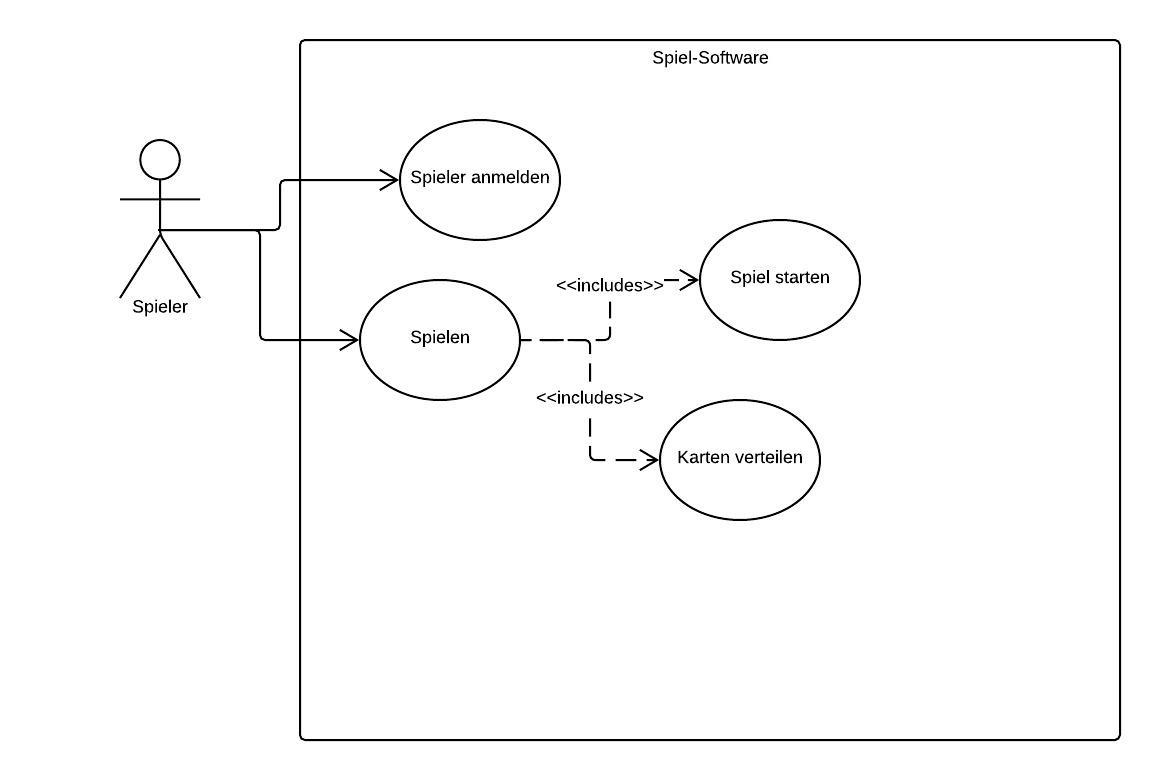
\includegraphics[width=0.9\textwidth]{img/ucd.jpg}
%\label{fig:systemgrenze}
%\caption{Ein Beispiel für Systemgrenzediagramm (Use Case Diagramm), das vor Abgabe anzupassen ist.}
%\end{figure}



	%gehört eher in das Pflichtenheft 
\section{Produktdaten}

Hier sollen die Daten genannt werden, die im System verwendet werden.

\newcounter{ld}\setcounter{ld}{10}

\begin{description}[leftmargin=5em, style=sameline]
	
	\begin{lhp}{ld}{LD}{daten:benutzername}
		\item [Name:] Benutzername*\footnote{``*'' bedeutet hier, dass die Daten in der Datenbank zu speichern sind}
		\item [Fachliche Beschreibung:] Benutzername des Spielers
		\item [Relevante Systemfunktionen:] \ref{funk:spielverw}, \ref{funk:zugriff}
	\end{lhp}
	
	\begin{lhp}{ld}{LD}{daten:passwort}
		\item [Name:] Passwort*
		\item [Fachliche Beschreibung:] Passwort des Spielers
		\item [Relevante Systemfunktionen:] \ref{funk:zugriff}
	\end{lhp}

	\begin{lhp}{ld}{LD}{daten:gewonneneSp}
		\item [Name:] Gewonnene Spiele*
		\item [Fachliche Beschreibung:] Anzahl der gewonnenen Spiele eines Spielers
		\item [Relevante Systemfunktionen:] \ref{funk:bestenliste}
	\end{lhp}

	\begin{lhp}{ld}{LD}{daten:spielzeit}
		\item [Name:] Spielzeit*
		\item [Fachliche Beschreibung:] Spielzeit eines Spielers, damit Eltern die Spielzeit ihrer Kinder einschränken können.
		\item [Relevante Systemfunktionen:] \ref{funk:zugriff}
	\end{lhp}

	\begin{lhp}{ld}{LD}{daten:taler}
		\item [Name:] Taler
		\item [Fachliche Beschreibung:] Taler eines Spielers
		\item [Relevante Systemfunktionen:] \ref{spielverw}
	\end{lhp}

	\begin{lhp}{ld}{LD}{daten:chat}
	\item [Name:] Chat
	\item [Fachliche Beschreibung:] Chatnachrichten innerhalb eines Chats.
	\item [Relevante Systemfunktionen:] \ref{chat}
	\end{lhp}

	\begin{lhp}{ld}{LD}{daten:bot}
	\item [Name:] Spielkarten
	\item [Fachliche Beschreibung:] Anzahl der ausgegebenen Spielkarten. Relevant für intelligente Bots.
	\item [Relevante Systemfunktionen:] \ref{bots}
	\end{lhp}

\end{description}
	\chapter{Nicht-funktionale Anforderungen}

\newcounter{nf}\setcounter{nf}{10}

\section{Softwarearchitektur}

\begin{description}[leftmargin=5em, style=sameline]	
	\begin{lhp}{nf}{NF}{nfunk:sarch1}
		\item [Name:] Client-Server Anwendung
		\item [Beschreibung:] Das verteilte Spiele-System ermöglicht das gemeinsame Spielen von verschiedenen Rechnern aus.
		\item [Motivation:] Aufgabestellung v. SEP/MP.
		\item [Erfüllungskriterium:] Das fertige System besteht aus Client- und Server-Teilen.
	\end{lhp}
	
	\begin{lhp}{nf}{NF}{nfunk:sarch1}
		\item [Name:] Plattformunabhängigkeit
		\item [Beschreibung:] Es soll sich um eine plattformunabhängige Anwendung handeln. Zumindest Windows- und Linuxsysteme sind zu unterstützen.
		\item [Motivation:] Aufgabenstellung v. SEP/MP.
		\item [Erfüllungskriterium:]In den Präsentationen kann der aktuelle Stand bzw. das fertige Produkt jederzeit vorgeführt werden.
	\end{lhp}
\end{description}



\section{Benutzerfreundlichkeit}


\begin{description}[leftmargin=5em, style=sameline]	
	\begin{lhp}{nf}{NF}{nfunk:alter}
		\item [Name:] Benutzeralter
		\item [Beschreibung:] Das System ist für Benutzer geeignet, die älter als 5 Jahre sind.
		\item [Motivation:] Jüngere Benutzer sind unfähig das Spiel zu spielen.
		\item [Erfüllungskriterium:] In AGB steht ein entsprechendes Hinweis.
	\end{lhp}
\end{description}

\begin{description}[leftmargin=5em, style=sameline]	
	\begin{lhp}{nf}{NF}{nfunk:keinetechniker}
		\item [Name:] Technische Fähigkeiten
		\item [Beschreibung:] Besondere technische Fähigkeiten sind von der Benutzern nicht zu erwarten.
		\item [Motivation:] Auch die Menschen, die kaum etwas von Bedienung bzw. Programmierung von Rechnern verstehen, sollen fähig sein, das System zu verwenden.
		\item [Erfüllungskriterium:]Jeder Benutzer kann die verschiedenen Funktionen intuitiv bedienen und spielen.
	\end{lhp}
\end{description}

\section{Leistungsanforderungen}

\begin{description}[leftmargin=5em, style=sameline]	
	\begin{lhp}{nf}{NF}{nfunk:antwortzeit}
		\item [Name:] Antwortzeit
		\item [Beschreibung:] Maximale Antwortzeit für alle Systemprozesse.
		\item [Motivation:] Das System muss immer brauchbar sein.
		\item [Erfüllungskriterium:] Das System antwortet auf Benutzerhandlungen nie später als in 10 Sekunden.
	\end{lhp}
\end{description}

\section{Anforderungen an Einsatzkontext}

\subsection{Anforderungen an physische Umgebung}

\begin{description}[leftmargin=5em, style=sameline]	
	\begin{lhp}{nf}{NF}{nfunk:beispiel1}
		\item [Name:] Lauffähigkeit an SCI-Rechnern
		\item [Beschreibung:] Das Produkt muss auf einem eigenem Geräte lauffähig sein, welches zur Präsentation am Ende des SEPs genutzt werden muss. Falls keine eigenen Rechner vorhanden, stehen auch die SCI-Terminals zur verfügung.
		\item [Motivation:] Optimierung von Betreuung und Abnahme des SEP/MP
		\item [Erfüllungskriterium:] Das fertige Produkt kann ohne Probleme an den vorhandenen Rechnern vorgeführt werden.
	\end{lhp}
\end{description}


%\subsection{Anforderungen an benachbarte Systeme}
%(sehe Systemkontext)
%
%\begin{description}[leftmargin=5em, style=sameline]	
%	\begin{lhp}{nf}{NF}{nfunk:beispiel2}
%		\item [Name:] Beispiel
%		\item [Beschreibung:] 
%		\item [Motivation:] 
%		\item [Erfüllungskriterium:] 
%	\end{lhp}
%\end{description}

\subsection{Absatz- sowie Installationsbezogene Anforderungen}

\begin{description}[leftmargin=5em, style=sameline]	
	\begin{lhp}{nf}{NF}{nfunk:beispiel3}
		\item [Name:] Installationsanleitung	
		\item [Beschreibung:] Falls die Installation nicht lediglich das Öffnen einer Datei voraussetzt, muss der genaue Installations- und Startvorgang schriftlich für Benutzer zur Verfügung gestellt.
		\item [Motivation:] Spezifikation
		\item [Erfüllungskriterium:] Eventuell auftretende Probleme bei der Installation können von jedem Nutzer anhand der Anleitung umgangen werden.
	\end{lhp}
\end{description}

\subsection{Anforderungen an Versionierung}

\begin{description}[leftmargin=5em, style=sameline]	
	\begin{lhp}{nf}{NF}{nfunk:beispiel4}
		\item [Name:] Keine weitere Versionen
		\item [Beschreibung:] Nach Version 1.0 keine weitere Entwicklung ist vorgesehen.
		\item [Motivation:] Das ist nur SEP/MP, keine Geschäftsprojekt, siehe \ref{fa:fortentwicklung}
		\item [Erfüllungskriterium:] Es werden keine Updates hinzugefügt.
	\end{lhp}
\end{description}

\section{Anforderungen an Wartung und Unterstützung}

\subsection{Wartungsanforderungen}

\begin{description}[leftmargin=5em, style=sameline]	
	\begin{lhp}{nf}{NF}{nfunk:beispiel4}
		\item [Name:] Wartung
		\item [Beschreibung:] Es ist keine Wartung von Seiten der Programmierer oder Dritter vorgesehen. 
		\item [Motivation:] Es sind weder Updates noch eine weitere Verwendung des Programms nach der Abnahme vorgesehen.
		\item [Erfüllungskriterium:] Das Programm wird nach der Abschlusspräsentation nicht weiterentwickelt.
	\end{lhp}
\end{description}

\begin{description}[leftmargin=5em, style=sameline]	
	\begin{lhp}{nf}{NF}{nfunk:doku}
		\item [Name:] Dokumentation
		\item [Beschreibung:] Der Quellcode muss ausführlich dokumentiert werden.
		\item [Motivation:] HiWis und der betreuende Professor sollen Entwicklungsschritte schneller nachvollziehen können.
		\item [Erfüllungskriterium:] JavaDoc 
	\end{lhp}
\end{description}

\begin{description}[leftmargin=5em, style=sameline]	
	\begin{lhp}{nf}{NF}{nfunk:doku}
		\item [Name:] Testen
		\item [Beschreibung:] Der Quellcode außer GUI muss gut getestet werden.
		\item [Motivation:] Fehler sollen frühzeitig erkannt und ausgebessert werden.
		\item [Erfüllungskriterium:] Von Unit-Tests muss mindestens 70\% des Quellcodes bedeckt werden. GUI-Klassen sind aus der Anforderung ausgenommen.
	\end{lhp}
\end{description}

\subsection{Anforderungen an technische und fachliche Unterstützung}

\begin{description}[leftmargin=5em, style=sameline]	
	\begin{lhp}{nf}{NF}{nfunk:beispiel5}
		\item [Name:] Beispiel
		\item [Beschreibung:] Keine technische und fachliche Unterstützung des Systems ist geplannt.
		\item [Motivation:] Siehe \ref{fa:fortentwicklung}.
		\item [Erfüllungskriterium:] Nicht anwendbar.
	\end{lhp}
\end{description}

\subsection{Anforderungen an technische Kompatibilität}

\begin{description}[leftmargin=5em, style=sameline]	
	\begin{lhp}{nf}{NF}{nfunk:beispiel6}
		\item [Name:] Technische Kompatibilität
		\item [Beschreibung:] Das Programm interagiert korrekt mit aller vorhergesehenen Soft- und Hardware.
		\item [Motivation:] Das Programm wird nicht von verschiedenen Kompatibilitätsfaktoren eingeschränkt.
		\item [Erfüllungskriterium:] Das Programm kann in den vorgegebenen Entwicklungsumgebungen eingesetzt werden.
	\end{lhp}
\end{description}

\section{Sicherheitsanforderungen}

\subsection{Zugang}

\begin{description}[leftmargin=5em, style=sameline]	
	\begin{lhp}{nf}{NF}{nfunk:beispiel7}
		\item [Name:] Zugang
		\item [Beschreibung:] Es wird nur Spielern Zugang gewährt, die ein registriertes Konto besitzen und sich darüber anmelden. 
		\item [Motivation:] Spieler und ihre Aktionen sollen auf ein Konto zurückverfolgbar sein.
		\item [Erfüllungskriterium:] Niemand kann die Software ohne gültigen Account nutzen.
	\end{lhp}
\end{description}

\subsection{Integrität}

\begin{description}[leftmargin=5em, style=sameline]	
	\begin{lhp}{nf}{NF}{nfunk:beispiel8}
		\item [Name:] Modifikation des Spiels
		\item [Beschreibung:] Spiele können nicht von anderen Spielern verändert werden.
		\item [Motivation:] Schummeln und Ärgern anderer Mitspieler ist unerwünscht.
		\item [Erfüllungskriterium:] Es wird bei der Implementierung auf gängige Sicherheitsverfahren geachtet. Die Spieler haben keine Möglichkeit, über die Programmoberfläche in den Quellcode des Spiels einzugreifen. 
	\end{lhp}
\end{description}

\subsection{Datenschutz/Privatsphäre}

\begin{description}[leftmargin=5em, style=sameline]	
	\begin{lhp}{nf}{NF}{nfunk:beispiel9}
		\item [Name:] Datenschutz/Privatsphäre
		\item [Beschreibung:] Private Spielerdaten sollen nicht von Dritten eingesehen oder für diese nutzbar gemacht werden.
		\item [Motivation:] Der Nutzer hat ein Recht darauf, dass die genutzte Software Datenschutz gewährleistet.
		\item [Erfüllungskriterium:] Es wird kein Rechtsbruch durch die Nutzung unserer Software auftreten.
	\end{lhp}
\end{description}


\subsection{Virenschutz}

\begin{description}[leftmargin=5em, style=sameline]	
	\begin{lhp}{nf}{NF}{nfunk:beispiel10}
		\item [Name:] Virenschutz
		\item [Beschreibung:] Es ist kein explizierter Virenschutz vorgesehen.
		\item [Motivation:] Die Software läuft lediglich über ein lokales Netzwerk, wodurch keine Malware von außen Einfluss nehmen kann.
		\item [Erfüllungskriterium:] Weder innerhalb unserer Software noch in anderen Programmen lassen sich Viren finden, die durch Sicherheitslücken in unserer Implementierung entstanden sind.
	\end{lhp}
\end{description}

\section{Prüfungsbezogene Anforderungen}

Anforderungen, die sich auf die Prüfung/Audit vom System von SEP/MP-Tutoren oder von weiteren Instanzen beziehen.


\begin{description}[leftmargin=5em, style=sameline]	
	\begin{lhp}{nf}{NF}{nfunk:beispiel10}
		\item [Name:] Formate der Systemdokumentation
		\item [Beschreibung:] Systemdokumantation muss in 2 Formen geführt werden (wenn anwendbar): Die Ausgangsdateien (\LaTeX, Dateien von Diagrammensoftware, von Grafiksoftware usw.) und PDFs.
		\item [Motivation:] Optimierung der SEP/MP-Betreuung.
		\item [Erfüllungskriterium:] Siehe Beschreibung.
	\end{lhp}
\end{description}

\section{Kulturelle und politische Anforderungen}


\begin{description}[leftmargin=5em, style=sameline]	
	\begin{lhp}{nf}{NF}{nfunk:beispiel11}
		\item [Name:] Systemsprache
		\item [Beschreibung:] Die Interfacesprache ist Deutsch.
		\item [Motivation:] Synchronisation des Verständnisses von Teammitgliedern mit unterschiedlichen kulturellen Hintergrunden.
		\item [Erfüllungskriterium:] Es tauchen keine weiteren Sprachen (Anglizismen ausgenommen) in der Software auf.
	\end{lhp}
\end{description}

\section{Rechtliche und standartsbezogene Anforderungen}


\begin{description}[leftmargin=5em, style=sameline]	
	\begin{lhp}{nf}{NF}{nfunk:beispiel12}
		\item [Name:] Nicht rechtliche Anforderungen
		\item [Beschreibung:] Es gibt keine relevanten rechtliche Anforderungen bekannt.
		\item [Motivation:] Siehe \ref{fa:fortentwicklung}.
		\item [Erfüllungskriterium:] Nicht anwendbar.
	\end{lhp}
\end{description}

	\chapter{Warteraum}

Hier werden Anforderungen spezifiziert die den sogenannten ``Warteraum'' darstellen. Hier gehören alle Anforderungen, die ``Wünschkriterien'' sind, das heißt, sie sind zwar erwünscht, aber werden nur dann in aktuelle Anforderungen übernommen, wenn dafür genügende Zeitbudget vorhanden ist und werden am wahrscheinlichsten in der Zukunft und nicht jetzt implementiert (oder in den kommenden Sprints beim SCRUM-Prozessmodell).

\newcounter{wr}\setcounter{wr}{10}

\begin{description}[leftmargin=5em, style=sameline]	
	\begin{lhp}{wr}{WR}{nfunk:sarch1}
		\item [Name:] Hintergrundmusik
		\item [Beschreibung:] Für die Spieler soll ein Auswahl zur Verfügung stehen, was für Hintergrundmusik sie beim Spielen in der Anwendung hören.
		\item [Motivation:] Höhere Zufriedenheit der Benutzer
		\item [Erfüllungskriterium:] Spieler können an jedem Zeitpunkt außer Vorraum aus einem Auswahl eine Musik auswählen oder die Musik ausschalten.
	\end{lhp}
\end{description}

\begin{description}[leftmargin=5em, style=sameline]	
	\begin{lhp}{wr}{WR}{nfunk:stats}
		\item [Name:] Stats der Spieler
		\item [Beschreibung:] In der Bestenliste soll es möglich sein, eine erweiterte Ansicht mit gewonnenen und verlorenen Spielen des Spielers zu sehen, sowie dessen höchst gewonnenes Spiel.
		\item [Motivation:] Höhere Zufriedenheit und mehr Ehrgeiz der Benutzer
		\item [Erfüllungskriterium:] Spieler können auf die Namen in der Bestenliste klicken.
	\end{lhp}
\end{description}

\begin{description}[leftmargin=5em, style=sameline]	
	\begin{lhp}{wr}{WR}{nfunk:freund}
		\item [Name:] Freundesliste
		\item [Beschreibung:] Es soll möglich sein, eine Freunde hinzuzufügen und zu sehen, ob diese online sind.
		\item [Motivation:] Höhere Zufriedenheit der Benutzer und mehr soziale Interaktion
		\item [Erfüllungskriterium:] Spieler können andere Spieler durch ein einen Button zur Freundesliste hinzufügen oder bestimmte Spielernamen suchen.
	\end{lhp}
\end{description}

\begin{description}[leftmargin=5em, style=sameline]	
	\begin{lhp}{wr}{WR}{nfunk:bots}
		\item [Name:] Bots
		\item [Beschreibung:] Es sollen mehr als zwei Schwierigkeitsstufen für Bots hinzugefügt werden.
		\item [Motivation:] Höhere Zufriedenheit der Benutzer
		\item [Erfüllungskriterium:] Spieler können aus mehreren Schwierigkeitsstufen für Bots wählen.
	\end{lhp}
\end{description}

\begin{description}[leftmargin=5em, style=sameline]	
	\begin{lhp}{wr}{WR}{nfunk:tut}
		\item [Name:] Tutorial
		\item [Beschreibung:] Beim ersten Login werden alle Menüpunkte durch Popups bzw. Tooltips erläutert.
		\item [Motivation:] Höhere Zufriedenheit der Benutzer und leichter Einstieg ins Spiel
		\item [Erfüllungskriterium:] Spieler erhalten beim ersten Login eine schrittweise Einführung in die Menüführung.
	\end{lhp}
\end{description}
\end{document}
